% Homework 5 - CS386(late submission)
% Russell Miller Winter 2011

\documentclass{article}
\usepackage{anysize}
\usepackage{wasysym}
\usepackage{graphicx}

\marginsize{2cm}{2cm}{2cm}{2cm}

\title{CS386 Homework 5}
\author{Russell Miller}
\date{\today}

\begin{document}

\maketitle

\section{}
\begin{description}
\item[a.]
ERD with cardinality constraints:\footnotemark\\
\footnotetext{ERDs drawn using Dia. http://projects.gnome.org/dia/\\
Edited with the GIMP [GNU Image Manipulation Program]}
\begin{center}
 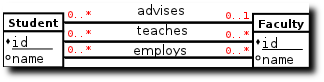
\includegraphics[scale=.8]{1a.png}
\end{center}
Relational Schema for this ERD:
\begin{quote}
\textbf{Student}(\underline{id}, name, advisor) advisor references Faculty.id\\
\textbf{Faculty}(\underline{id}, name)\\
\textbf{Teachers}(\underline{faculty\_id, student\_id}) faculty\_id references Faculty.id, student\_id 
references Student.id\\
\textbf{Employments}(\underline{faculty\_id, student\_id}) faculty\_id references Faculty.id, student\_id 
references Student.id\\
\end{quote}

\item[b.]
ERD with cardinality contraints:\\
\begin{center}
 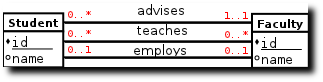
\includegraphics[scale=.8]{1b.png}
\end{center}
Relational Schema:
\begin{quote}
\textbf{Student}(\underline{id}, name, advisor, employer) advisor not null and references Faculty.id, employer references Faculty.id\\
\textbf{Faculty}(\underline{id}, name, employee) employee references Student.id\\
\textbf{Teachings}(\underline{faculty\_id, student\_id}) faculty\_id references Faculty.id, student\_id
references Student.id\\
\end{quote}
\end{description}

\section{}
\begin{description}
\item[a.]
\textbf{\\Person\\}
$id \rightarrow id\; ssn\; name\; phone$\\
$ssn \rightarrow id\; ssn\; name\; phone$\\
\textbf{PolicyOwner\\}
$Personid\; PolicyNumber \rightarrow SSN\; Start$-$date$\\
$PolicyNumber\; SSN \rightarrow Personid\; Start$-$date$\\
\textbf{InsurancePolicy\\}
$PolicyNumber \rightarrow AgentNumber\; AgentName\; Premium$
\item[b.]
\textbf{\\Person\\}
$id \rightarrow id$\\
$ssn \rightarrow ssn$\\
$id\; name \rightarrow name$\\
$ssn\; name \rightarrow name$\\
$id\; phone \rightarrow phone$\\
\textbf{PolicyOwner\\}
$Personid\; PolicyNumber \rightarrow Personid\; PolicyNumber$\\
$PolicyNumber\; SSN \rightarrow PolicyNumber\; SSN$\\
$Personid\; PolicyNumber\; SSN \rightarrow SSN$\\
$Personid\; PolicyNumber\; SSN \rightarrow Personid$\\
$PolicyNumber\; SSN\; Start$-$date \rightarrow Start$-$date$\\
\textbf{InsurancePolicy\\}
$PolicyNumber \rightarrow PolicyNumber$\\
$PolicyNumber\; AgentNumber \rightarrow AgentNumber$\\
$PolicyNumber\; AgentName \rightarrow AgentName$\\
$PolicyNumber\; Premium \rightarrow Premium$\\
$PolicyNumber\; AgentNumber\; AgentName \rightarrow AgentName$\\
\item[c.]
\textbf{\\Person\\}
$none$\\
\textbf{PolicyOwner\\}
$Personid \rightarrow SSN$\\
$SSN \rightarrow Personid$\\
\textbf{InsurancePolicy\\}
$AgentNumber \rightarrow AgentName$
\item[d.]
\textbf{\\Person\\}
N/A\\
\textbf{PolicyOwner\\}
Because of the redundancy of the SSN field between the Person table and the
PolicyOwner table, iff the SSN field is updated in either table, there may
be a discrepancy between the values in the tables, when they should match.\\
\textbf{InsurancePolicy\\}
If an AgentNumber or AgentName change for a specific insurance agent, and
more than one policy has the same agent, it's possible that the rows, which
should have matching AgentNumbers and AgentNames, could have a discrepancy.

\pagebreak

\item[e.]
\textbf{\\Person}(\underline{id}, ssn, name, phone)\\
\textbf{PolicyOwner}(\underline{Personid, PolicyNumber}, Start-date) Personid 
references Person.id and PolicyNumber references InsurancePolicy.PolicyNumber\\
\textbf{InsurancePolicy}(\underline{PolicyNumber}, AgentNumber, Premium) 
AgentNumber references Agent.id\\
\textbf{Agent}(\underline{id}, name)
\end{description}

\section{}
\begin{description}
\item[a.]
\ \\
Student(\underline{id}, student-name, phone, major)\\
Advisor(\underline{student-name, advisor-id}, advisor-name) student-name references
Student.student-name\\
\item[b.]
\textbf{\\Original Table:\\}
\begin{tabular}{l|l|l|l|l|l}
id & name & phone    & advisor-id & advisor-name & major\\
\hline
1  & Mary  & 555-1111 & 1          & Aren         & Dancing\\
2  & Ben   & 555-0121 & 2          & Justin       & Basketweaving\\
3  & Mary  & 555-3345 & 3          & Wendy        & History\\
4  & David & 555-9987 & 4          & Adam         & Sniper\\
\end{tabular}
\textbf{\\Student Table:\\}
\begin{tabular}{l|l|l|l}
id & student-name & phone    & major\\
\hline
1  & Mary         & 555-1111 & Dancing\\
2  & Ben          & 555-0121 & Basketweaving\\
3  & Mary         & 555-3345 & History\\
4  & David        & 555-9987 & Sniper\\
\end{tabular}
\textbf{\\Advisor Table:\\}
\begin{tabular}{l|l|l}
student-name & advisor-id & advisor-name\\
\hline
Mary         & 1          & Aren\\
Ben          & 2          & Justin\\
Mary         & 3          & Wendy\\
David        & 4          & Adam\\
\end{tabular}
\item[c.]
\ \\
\begin{tabular}{l|l|l|l|l|l}
id & student-name & phone    & major         & agent-id & agent-name\\
\hline
1  & Mary         & 555-1111 & Dancing       & 1        & Aren\\
1  & Mary         & 555-1111 & Dancing       & 3        & Wendy\\
2  & Ben          & 555-0121 & Basketweaving & 2        & Justin\\
3  & Mary         & 555-3345 & History       & 1        & Aren\\
3  & Mary         & 555-3345 & History       & 3        & Wendy\\
4  & David        & 555-9987 & Sniper        & 4        & Adam\\
\end{tabular}
\end{description}
\end{document}
